\documentclass{standalone}
\usepackage{tikz}
\usetikzlibrary{arrows, calc}
\begin{document}

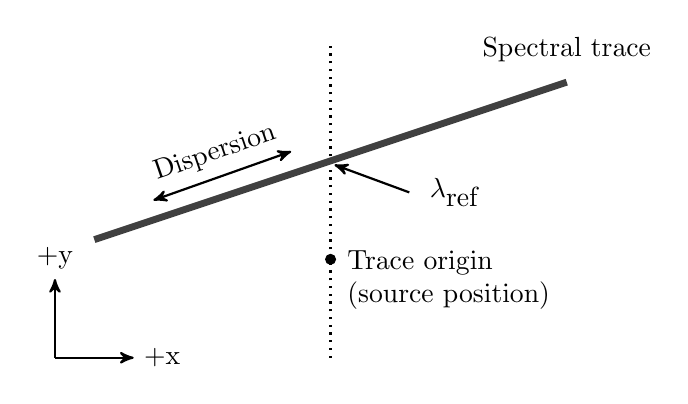
\begin{tikzpicture}[
    scale=1,
    thick,
    >=stealth']


    % origin
    \draw[->] (0,0) -- (1,0) coordinate[label={right:+x}];
    \draw[->] (0,0) -- (0,1) coordinate[label={above:+y}];
    
    % reference line
    %\draw[dotted] (3.5,0) node [below] {$x_{\mbox{ref}}$} -- (3.5,4);
    \draw[dotted] (3.5,0) -- (3.5,4);
    
    % source location
    \node at (5, 1) {\begin{tabular}{l} Trace origin \\ (source position) \end{tabular}};
    %\node[label={right:Source position}] at (3.5,1.25) {};
    \fill[black] (3.5,1.25) circle(2pt);

    % spectrum
    \draw[line width=2.5pt, color=darkgray] (0.5,1.5) -- (6.5,3.5);
    \node[label={above:Spectral trace}] at (6.5,3.5) {};
    %\node at (6.33,3) {\begin{tabular}{l} Spectral \\ trace \end{tabular}};


    % dispersion direction
    \draw[<->] (1.25,2) -- (3,2.62);
    \node[label={[rotate=19]above:Dispersion}] at (2.125,2.2) {};

    % trace origin
    \draw[<-] (3.55,2.45) -- (4.5,2.1);
    \node[label={right:$\lambda_{\mbox{ref}}$}] at (4.5,2.1) {};
    
    
    
    
    
    %\draw[<-] (2.7,3.3) -- (3.6,3.7);
    %\node[label={[rotate=20]above:Dispersion direction}] at (3.1,3.5) {};

    %\draw[<-] (2.3215,1.9286) -- (3.25,2.3);
    %\node[label={above:$+d$}] at (2.75,2.05) {};
    %\draw[->] (3.35,2.35) -- (4.2785,2.7214);
    %\node[label={above:$-d$}] at (3.67,2.42) {};
    
    %\draw[<-] (2.7858,2.1143) -- (3.25,2.3);
    %\node[label={[rotate=20]left:$d>0$}] at (2.88,2.14) {};
    %\draw[->] (3.35,2.35) -- (3.8142,2.5357);
    %\node[label={[rotate=20]right:$d<0$}] at (3.7, 2.58) {};


\end{tikzpicture}
\end{document}